% Include from the sabmod repository root with graphicx loaded.
% Call \showscriptprovenancefalse to hide script provenance.
\newif\ifshowscriptprovenance
\showscriptprovenancetrue
\providecommand{\scriptprovenance}[1]{%
  \ifshowscriptprovenance\space Scripts: \texttt{\detokenize{#1}}.\fi}

\begin{figure}[htbp]
  \centering
  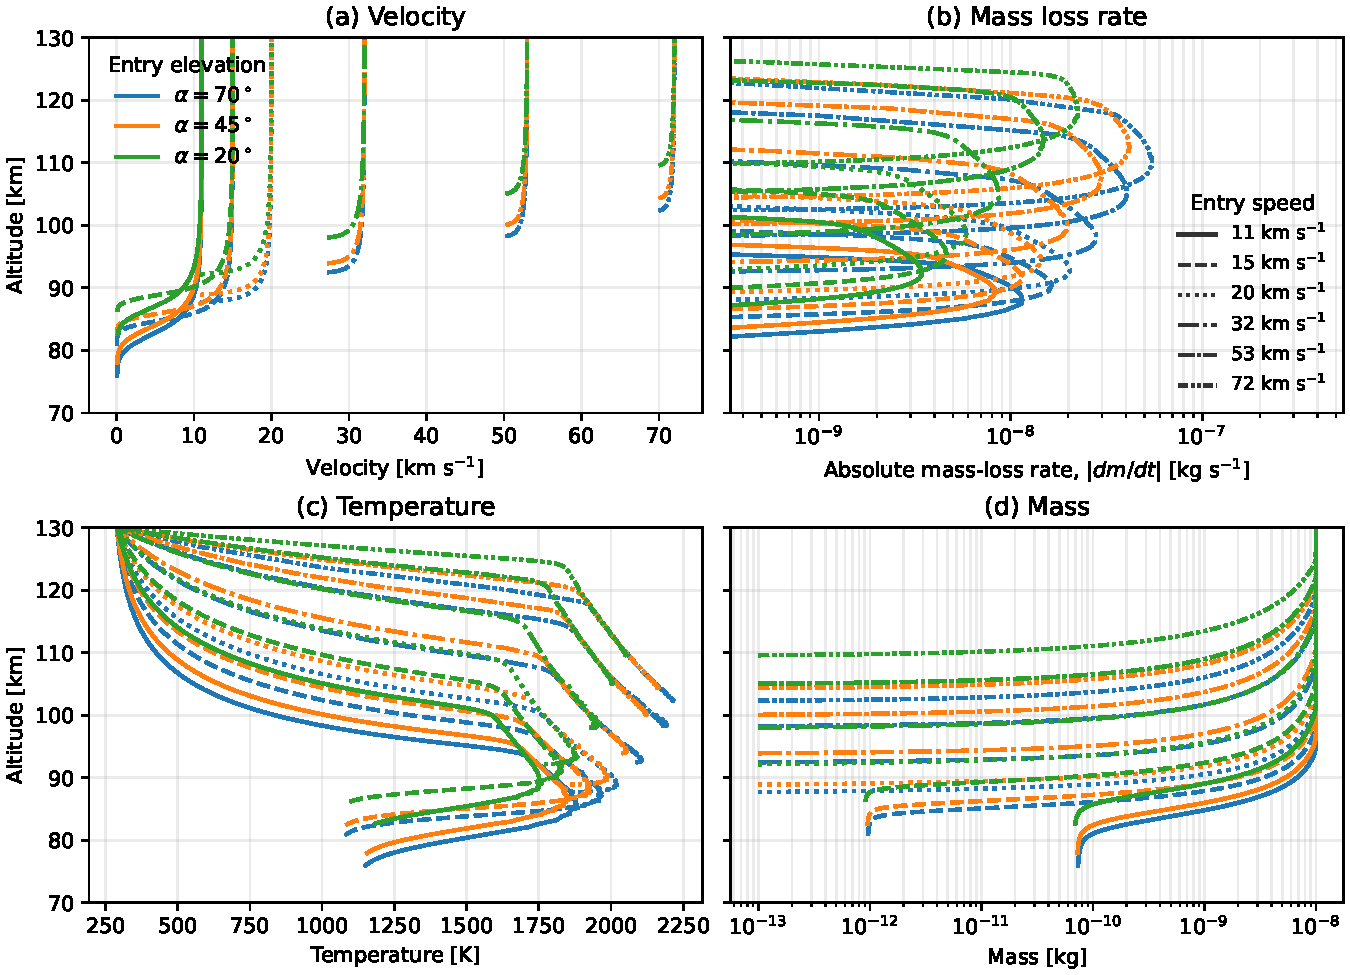
\includegraphics[width=\linewidth]{reproduction_extended/figures/meteor_ablation_single_column.pdf}
  \caption{Extended ablation profiles for $10^{-8}$~kg cometary particles
  at entry speeds of 11, 15, 20, 32, 53, and 72~km~s$^{-1}$. Entry
  elevation angles above the horizon are $70^\circ$, $45^\circ$, and
  $20^\circ$. The atmosphere and equations follow the paper reproduction;
  the maximum integration duration is increased to 30~s to capture the
  low-speed peaks.
  \scriptprovenance{reproduce_paper.py; extended_paper_plots.py;
  paper/make_cabmod_figures.py}}
\end{figure}

\begin{figure}[htbp]
  \centering
  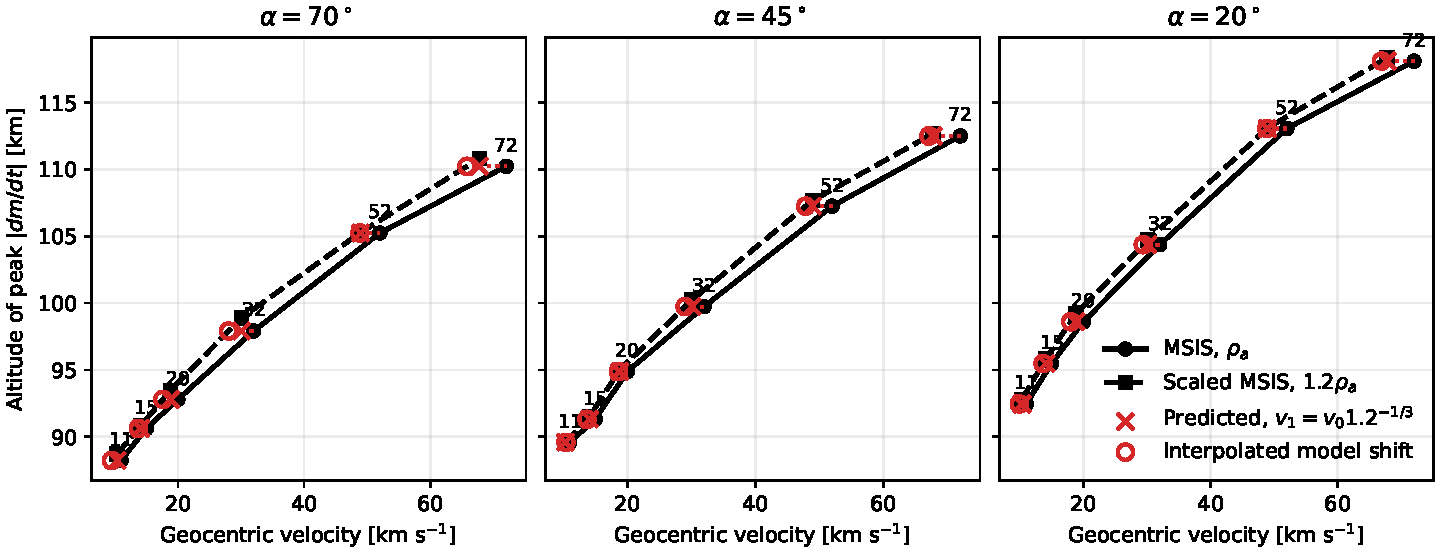
\includegraphics[width=\linewidth]{reproduction_extended/figures/peak_ablation_height-1.20.pdf}
  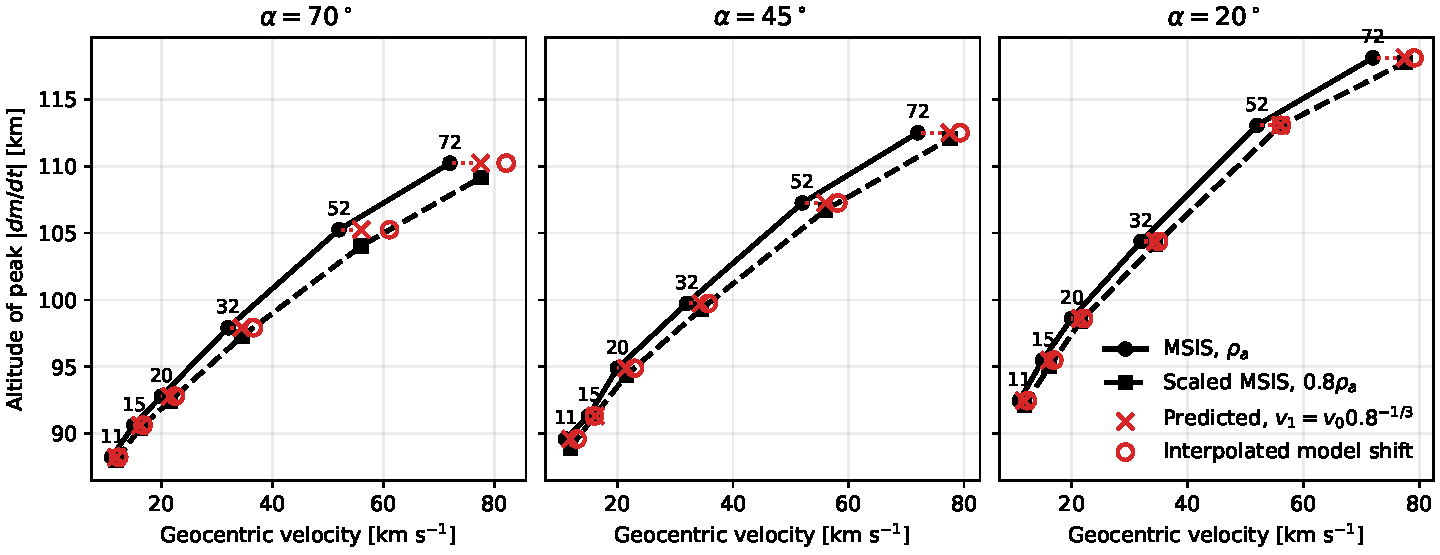
\includegraphics[width=\linewidth]{reproduction_extended/figures/peak_ablation_height-0.80.pdf}
  \caption{Extended peak mass-loss altitude comparison for atmospheric
  density factors 1.2 (top) and 0.8 (bottom), with entry elevation angles
  shown in columns. Baseline speeds are 11, 15, 20, 32, 52, and
  72~km~s$^{-1}$. Red crosses show the simple cubic velocity-scaling
  prediction; open circles show the model shift inferred using the
  expanded piecewise-linear height-to-velocity mapping.
  \scriptprovenance{reproduce_paper.py; extended_paper_plots.py;
  paper/make_cabmod_figures.py}}
\end{figure}

\begin{figure}[htbp]
  \centering
  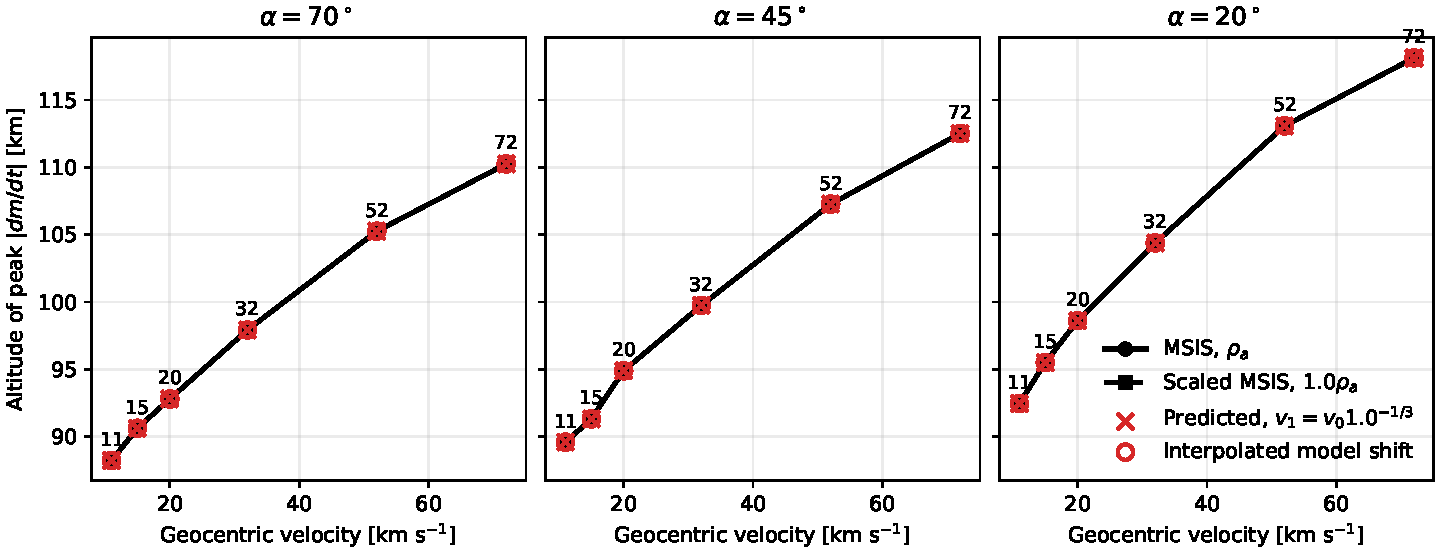
\includegraphics[width=\linewidth]{reproduction_extended/figures/peak_ablation_height-1.00.pdf}
  \caption{Unscaled atmosphere control for the extended entry-speed family.
  \scriptprovenance{reproduce_paper.py; extended_paper_plots.py;
  paper/make_cabmod_figures.py}}
\end{figure}
